\section{Projekt Narra}
\par Narra je projekt s volně dostupným zdrojovým kódem, který se zabývá anotací a propojením audiovizuálních médií a textu. Podobně jako YouTube má také veřejně dostupné API po dokončení souží umělcům, filmařům a dalším, kteří chtějí vytvářet otevřený příběh (open narrative), nebo editovat videa. Dokumentaristé mohou tento projekt využít pro rozsáhlejší díla, díky nabídnutému relevantnímu obsahu s metadaty. Projekt zastřešuje FAMU CAS, které poskytuje práci pro více jak 30 studentů dokončujících Bakalářské a Magisterské studium.
\par S první myšlenkou projektu Narra přišel v roce 2002 - 2003 Eric Rosenzveig a Willy LeMaitre spolu s dalšími mediálními umělci a programátory. Dílo bylo rozdělené na tři části. První "plaListNetWork" byl opensource software vyvinutý na základě konzultací s umělci o audiovizuálním obsahu a rozhraním pro vizualizaci. Umožňoval práci více uživatelů na různých místech a pomocí textových poznámek upravovat popisky skladeb a videí. Druhý "disPlayList" bylo veřejně přístupné rozhraní pro streamování medií z playListNetWork. Jednalo se o webovou aplikaci, která vizualizovala výsledná videa do grafu, ze kterého šel pomocí klíčových slov tvořit další celek. "Ressemblage", neboli poslední část byl výsledkem práce umělců používajících novou technologii práce s médii.
\par V projekt Open Narrative se zapříčinil nejvíce umělec Eric Rosenzveig a reaktor Tomáš Dobruška na FAMU v letech 2010 - 2015. Díky penězům z grantu mohou pokračovat ve vývoji spolu s katedrou KSI FIT ČVUT.

\section{Technologie v projektu Narra} 
\par Narra je psaná v jazyce Ruby a poskytuje REST-API pro komunikaci se světem. Další použité technologie jsou Sidekiq, OmniAuth, MongoDB a Rails. Všechny tyto komponenty zajišťují stabilní jádro aplikace, na které je možné připisovat další balíčky (gem), jako v případě mé bakalářské práce. Pro začátek jsem se musel seznámit s databázovám modelem celé aplikace.

\begin{figure}[h]
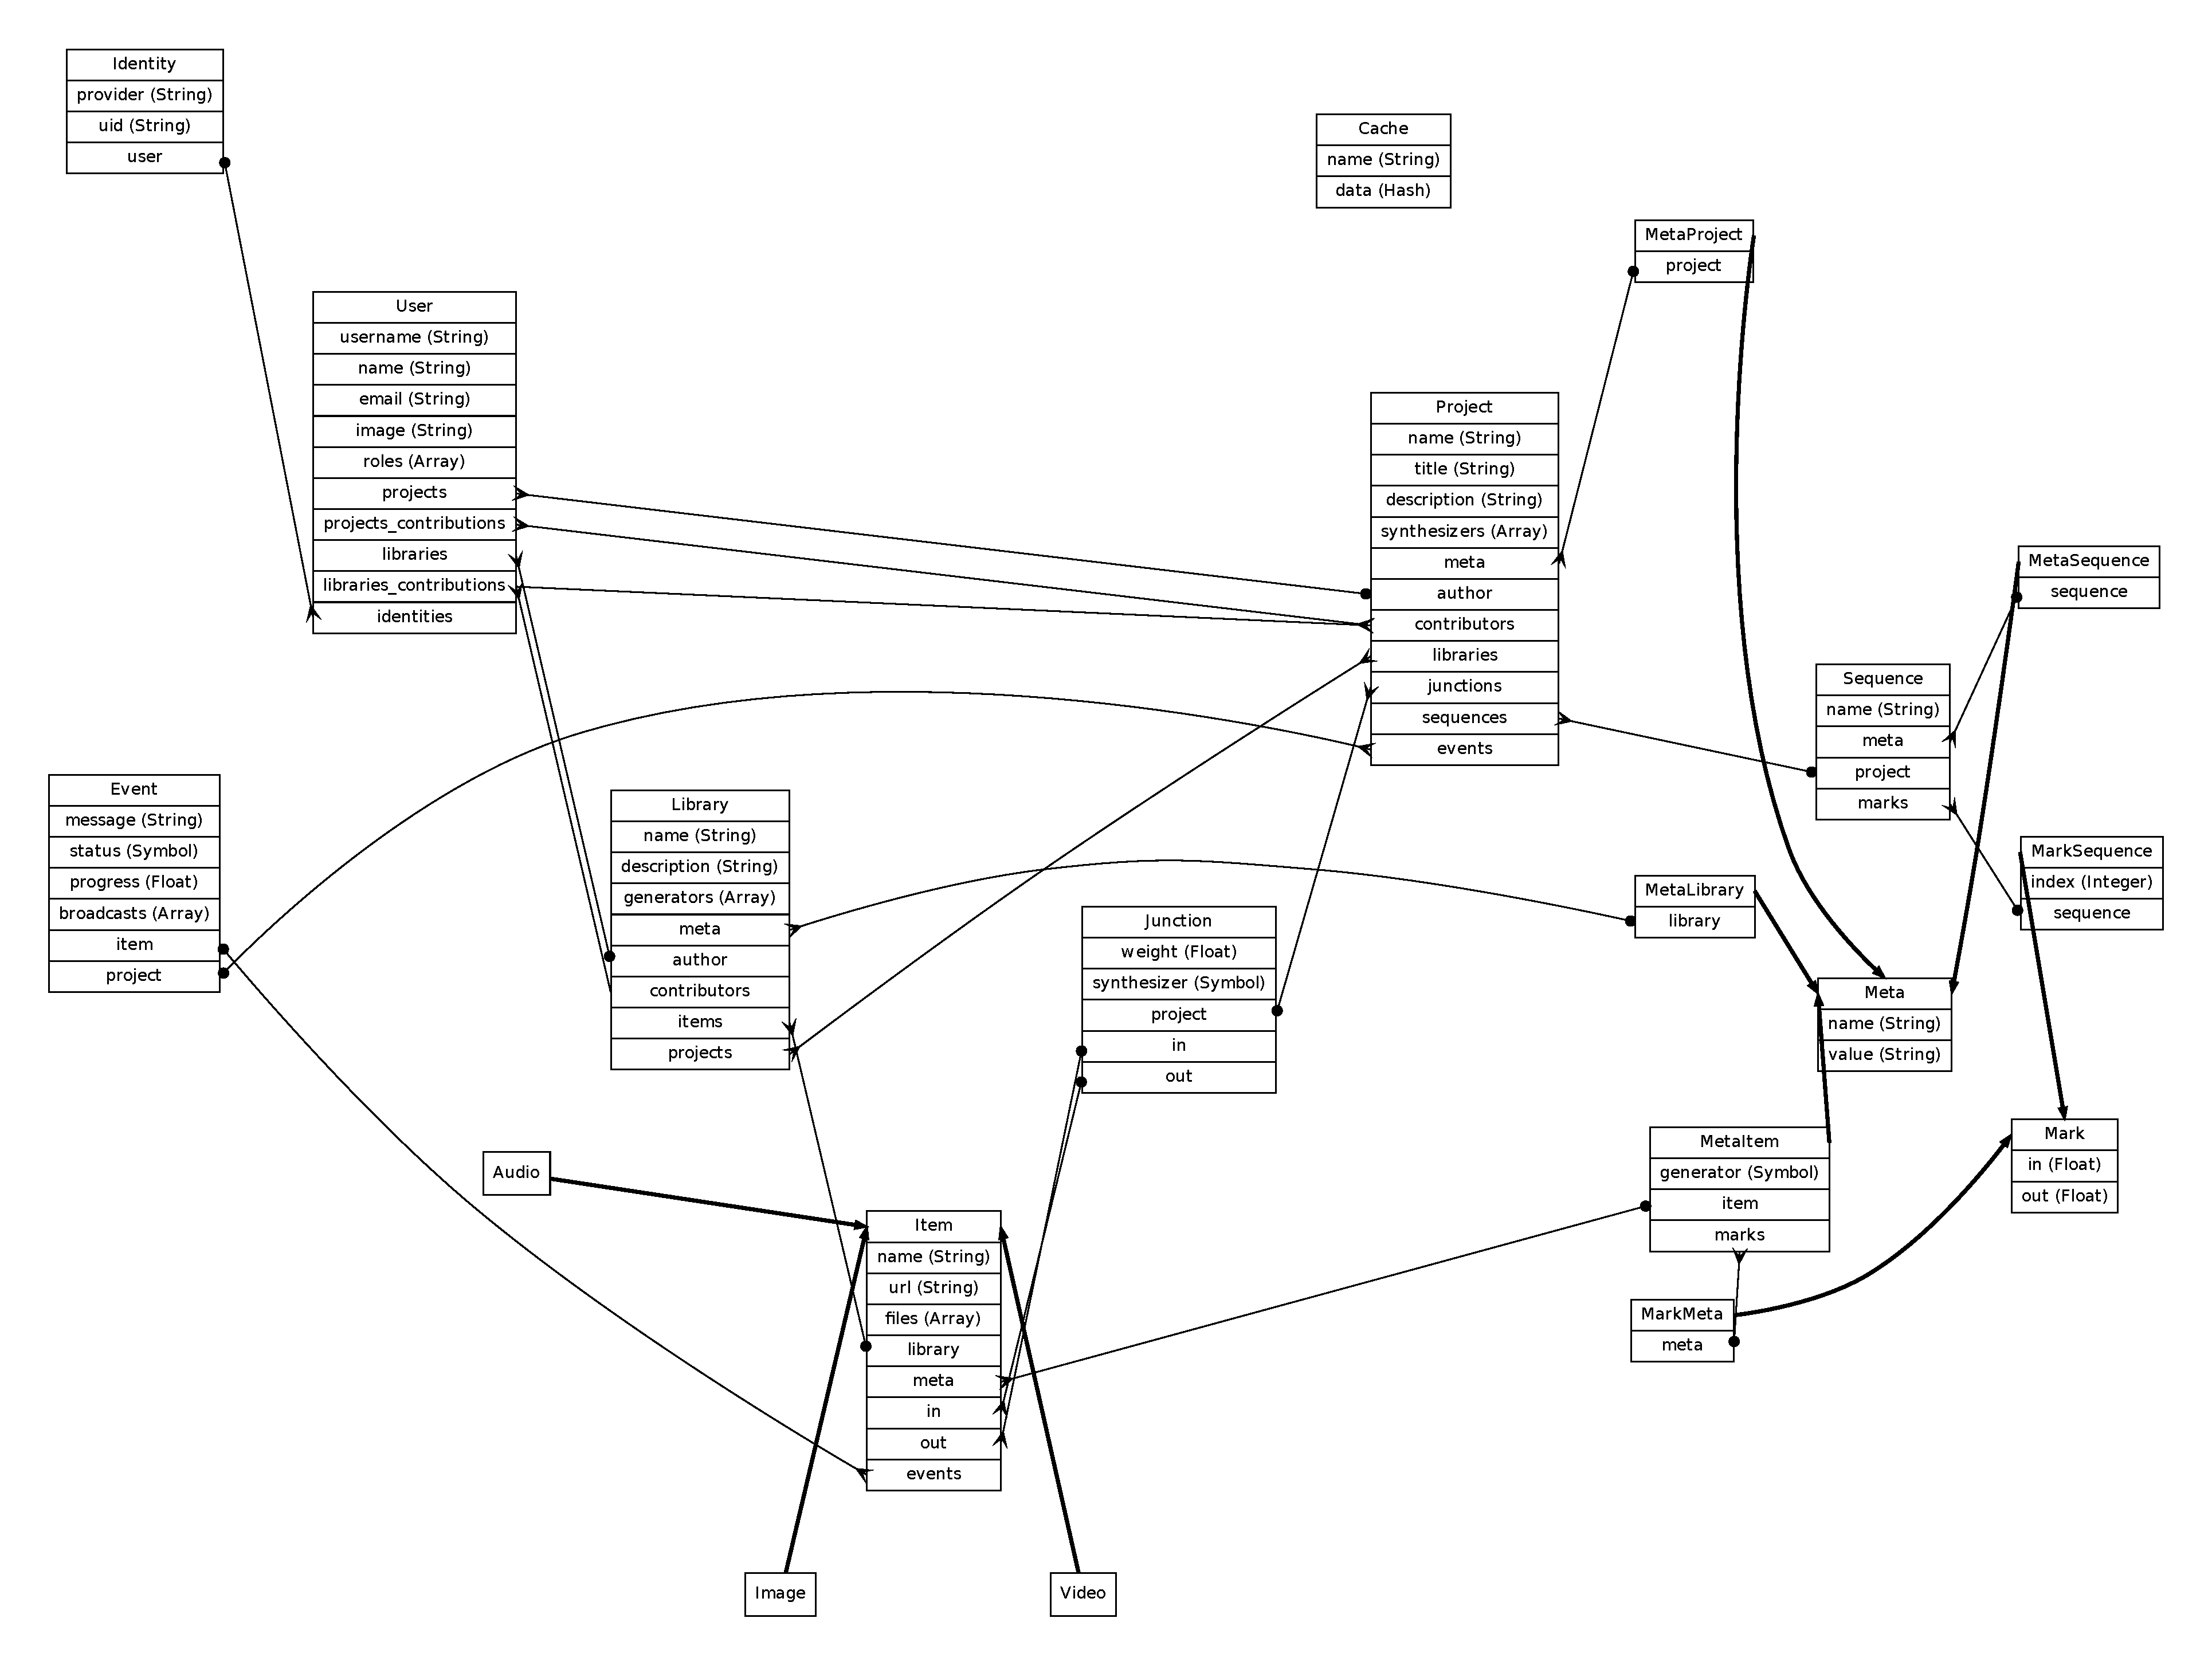
\includegraphics{./obrazova_priloha/domain_full.pdf}
\caption{Doménový model Narra}
\end{figure}

\par Z celého doménového modelu mě zajímají Meta, MetaItem, MarkMeta a Item.
// todo

\begin{figure}[h]
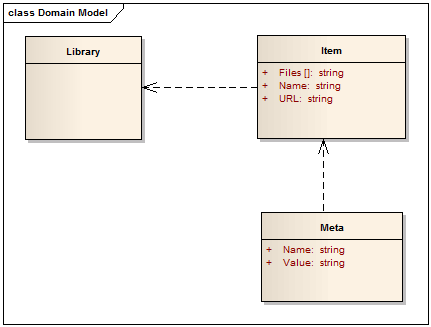
\includegraphics{./obrazova_priloha/domain_my.png}
\caption{Část na kterou navazuji Narra}
\end{figure}
\par // toho popis
